\documentclass[10pt,letterpaper]{article}
\usepackage[T1]{fontenc}
\usepackage{times,microtype}
\usepackage[utf8]{inputenc}
\usepackage[margin=.8in]{geometry}
\usepackage{booktabs,amsmath,amssymb,graphicx,array,pdfpages}
\usepackage[hidelinks]{hyperref}
\newcommand{\APlit}{\mathrm{AP}_{\mathrm{toolkit}}}
\renewcommand{\thetable}{S\arabic{table}}
\renewcommand{\thefigure}{S\arabic{figure}}
\title{Supplementary Results for HyCADO}
\author{Gul Erten and Mehmet Koc}
\date{}
\begin{document}
\maketitle
These materials accompany \emph{HyCADO for Detector-Guided Region Refinement in UAV Object Detection}. They retain the completed COCO-style evaluation, paired uncertainty, operating-point diagnostics, and fixed-sample qualitative atlas, together with the historical toolkit and VAL diagnostic results. Numerical tables are regenerated from completed stages 22--24 and 28--30; the fixed-sample qualitative atlas and its selection records come from stage 25. No training, new inference, or parameter selection was performed when preparing this revision.

\section{Metric definitions and scope}
COCO-style bbox AP uses \texttt{pycocotools} 2.0.11 with native coordinates, ten IoU thresholds from 0.50 to 0.95, 101 recall thresholds, and equal-class averaging. The pinned VisDrone category-zero ignore-map preprocessing applies to GT and detections before evaluation. The retained input contains 38599 normal targets on VAL and 74707 on test-dev. No class-specific score-zero target remains in these evaluated inputs. Frozen final scores and candidates are reused without a new display threshold or NMS.

The primary COCO limit is maxDets100 per image and category. The maxDets500 sensitivity uses the same inputs. No historical global max500 truncation is applied before these evaluations, and SAHI candidate lists are not capped at 1000 on ingestion. Area ranges use the upstream boundaries at $32^2$ and $96^2$ native pixels$^2$, including its boundary conventions. AR uses the displayed cap. Area-specific and cap500 results are point estimates without confidence intervals.

Historical toolkit AP, its equal-class macro diagnostic, and COCO-style AP are distinct quantities. Recall--FP curves use toolkit-aligned matching with a global max500 cap and are not COCO AR. All AP/recall values use a 0--100 scale and differences are points. Test-dev intervals use 1000 paired draws over 61 filename/hash proxy groups, conditional on one trained model set. These groups are not verified independent scenes. Secondary intervals are marginal and unadjusted. The resolution, COCO, SAHI, two-resolution fusion, and multiplier/geometry extensions followed earlier test-dev analysis and provide no new untouched confirmation set.

\section{COCO-style point results}
No HyCADO-1280 VAL COCO result is available in this bounded extension; its full evaluation is on test-dev. The three test-dev relocation conditions retain the original HyCADO-800 geometry and crop network. They are separate placement scores, not an ensemble. In every table, a SAHI suffix specifies native slice side length; the detector target remains 800 with the same YOLO checkpoint.
\begin{table}[h!]
\centering\footnotesize\setlength{\tabcolsep}{4pt}
\caption{VAL COCO-style point metrics, maxDets100.}
\begin{tabular}{lrrrrrrr}
\toprule
Method & AP & AP$_{50}$ & AP$_{75}$ & AP$_S$ & AP$_M$ & AP$_L$ & AR$_{100}$\\
\midrule
YOLO-800 & 27.603 & 44.994 & 28.126 & 18.145 & 40.253 & 49.171 & 37.484\\
YOLO-1280 & 31.095 & 51.014 & 31.821 & 23.649 & 40.947 & 37.404 & 42.970\\
YOLO-1536 & 30.016 & 49.798 & 30.431 & 23.829 & 38.350 & 31.109 & 42.891\\
SAHI-640 + YOLO & 31.433 & 52.160 & 31.793 & 24.972 & 41.166 & 44.644 & 46.456\\
SAHI-800 + YOLO & 30.932 & 50.763 & 31.549 & 22.827 & 41.397 & 49.230 & 43.817\\
HyCADO-800 & 29.457 & 47.948 & 30.051 & 20.285 & 41.577 & 50.956 & 44.320\\
\bottomrule
\end{tabular}

\end{table}
\clearpage
\begin{table}[t]
\centering\footnotesize\setlength{\tabcolsep}{3.6pt}
\caption{Test-dev COCO-style point metrics, maxDets100. Regions 800 / global 1280 is the mixed-resolution refinement variant.}
\begin{tabular}{lrrrrrrr}
\toprule
Method & AP & AP$_{50}$ & AP$_{75}$ & AP$_S$ & AP$_M$ & AP$_L$ & AR$_{100}$\\
\midrule
YOLO-800 & 21.476 & 35.765 & 22.240 & 10.983 & 32.133 & 43.000 & 31.783\\
YOLO-1280 & 23.996 & 40.230 & 24.425 & 15.365 & 33.295 & 35.016 & 36.166\\
HyCADO-800 & 22.377 & 37.269 & 23.153 & 12.084 & 32.844 & 42.982 & 36.332\\
Relocation seed 0 & 21.428 & 35.592 & 22.217 & 11.133 & 31.973 & 42.150 & 32.916\\
Relocation seed 1 & 21.405 & 35.523 & 22.201 & 11.116 & 31.961 & 42.257 & 32.797\\
Relocation seed 2 & 21.430 & 35.586 & 22.213 & 11.183 & 31.888 & 41.916 & 32.933\\
HyCADO-1280 & 24.435 & 40.804 & 24.940 & 15.906 & 33.832 & 34.910 & 39.128\\
HyCADO, regions 800 / global 1280 & 24.469 & 40.880 & 24.974 & 15.916 & 33.892 & 34.909 & 39.237\\
SAHI-640 + YOLO & 24.529 & 41.623 & 24.922 & 15.692 & 32.793 & 41.419 & 39.817\\
\bottomrule
\end{tabular}

\end{table}
\begin{table}[h!]
\centering\footnotesize\setlength{\tabcolsep}{4pt}
\caption{VAL COCO-style sensitivity, maxDets500.}
\begin{tabular}{lrrrrrrr}
\toprule
Method & AP & AP$_{50}$ & AP$_{75}$ & AP$_S$ & AP$_M$ & AP$_L$ & AR$_{500}$\\
\midrule
YOLO-800 & 27.647 & 45.081 & 28.163 & 18.189 & 40.308 & 49.170 & 37.656\\
YOLO-1280 & 31.181 & 51.255 & 31.884 & 23.738 & 41.077 & 37.402 & 43.294\\
YOLO-1536 & 30.118 & 50.044 & 30.500 & 23.933 & 38.516 & 31.297 & 43.309\\
SAHI-640 + YOLO & 31.513 & 52.411 & 31.820 & 25.060 & 41.215 & 44.644 & 46.702\\
SAHI-800 + YOLO & 30.989 & 50.955 & 31.555 & 22.892 & 41.439 & 49.231 & 43.958\\
HyCADO-800 & 29.588 & 48.220 & 30.150 & 20.432 & 41.669 & 50.969 & 45.228\\
\bottomrule
\end{tabular}

\end{table}
\begin{table}[h!]
\centering\footnotesize\setlength{\tabcolsep}{3.6pt}
\caption{Test-dev COCO-style sensitivity, maxDets500.}
\begin{tabular}{lrrrrrrr}
\toprule
Method & AP & AP$_{50}$ & AP$_{75}$ & AP$_S$ & AP$_M$ & AP$_L$ & AR$_{500}$\\
\midrule
YOLO-800 & 21.530 & 35.917 & 22.280 & 11.038 & 32.189 & 42.998 & 31.985\\
YOLO-1280 & 24.085 & 40.521 & 24.455 & 15.454 & 33.426 & 35.139 & 36.529\\
HyCADO-800 & 22.488 & 37.558 & 23.211 & 12.201 & 32.934 & 42.990 & 37.304\\
Relocation seed 0 & 21.511 & 35.810 & 22.260 & 11.219 & 32.035 & 42.155 & 33.467\\
Relocation seed 1 & 21.489 & 35.751 & 22.244 & 11.200 & 32.019 & 42.259 & 33.364\\
Relocation seed 2 & 21.510 & 35.806 & 22.255 & 11.268 & 31.952 & 41.921 & 33.451\\
HyCADO-1280 & 24.564 & 41.138 & 25.012 & 16.047 & 33.940 & 34.996 & 40.144\\
HyCADO, regions 800 / global 1280 & 24.600 & 41.225 & 25.049 & 16.056 & 34.013 & 34.984 & 40.253\\
SAHI-640 + YOLO & 24.630 & 41.941 & 24.962 & 15.794 & 32.901 & 41.419 & 40.204\\
\bottomrule
\end{tabular}

\end{table}
\clearpage
\section{Paired test-dev COCO contrasts}
The resolution analysis prespecified HyCADO-1280 minus YOLO-1280 as its primary COCO contrast. The later SAHI extension prespecified HyCADO-1280 minus SAHI-640 and reused identical comparator draws. The table retains all five contrasts and four evaluated metrics. Bounds are the linear 2.5th and 97.5th percentiles of paired differences. The check script recomputes bounds and bootstrap standard errors from retained draws. An interval crossing zero establishes neither equivalence nor superiority.
\begin{table}[h!]
\centering\footnotesize\setlength{\tabcolsep}{3.5pt}
\caption{Paired test-dev COCO differences at maxDets100. The two primary roles refer to the separately recorded resolution and SAHI protocols. All intervals are marginal 95\% intervals.}
\begin{tabular}{llrr}
\toprule
Contrast & Metric & $\Delta$ & 95\% interval\\
\midrule
HyCADO-1280 $-$ YOLO-1280 & AP & +0.439 & [+0.161, +0.838]\\
HyCADO-1280 $-$ YOLO-1280 & AP50 & +0.574 & [+0.041, +1.229]\\
HyCADO-1280 $-$ YOLO-1280 & AP75 & +0.515 & [+0.240, +0.969]\\
HyCADO-1280 $-$ YOLO-1280 & AR100 & +2.961 & [+2.352, +4.130]\\
HyCADO-1280 $-$ SAHI-640 & AP & -0.095 & [-0.776, +0.743]\\
HyCADO-1280 $-$ SAHI-640 & AP50 & -0.819 & [-1.858, +0.553]\\
HyCADO-1280 $-$ SAHI-640 & AP75 & +0.018 & [-0.775, +0.950]\\
HyCADO-1280 $-$ SAHI-640 & AR100 & -0.689 & [-1.713, +0.769]\\
SAHI-640 $-$ YOLO-1280 & AP & +0.534 & [-0.078, +1.154]\\
SAHI-640 $-$ YOLO-1280 & AP50 & +1.393 & [+0.318, +2.385]\\
SAHI-640 $-$ YOLO-1280 & AP75 & +0.497 & [-0.139, +1.270]\\
SAHI-640 $-$ YOLO-1280 & AR100 & +3.651 & [+2.911, +4.561]\\
Regions 800 / global 1280 $-$ YOLO-1280 & AP & +0.473 & [+0.199, +0.857]\\
Regions 800 / global 1280 $-$ YOLO-1280 & AP50 & +0.650 & [+0.142, +1.291]\\
Regions 800 / global 1280 $-$ YOLO-1280 & AP75 & +0.550 & [+0.278, +0.984]\\
Regions 800 / global 1280 $-$ YOLO-1280 & AR100 & +3.071 & [+2.470, +4.223]\\
HyCADO-1280 $-$ regions 800 / global 1280 & AP & -0.034 & [-0.075, +0.017]\\
HyCADO-1280 $-$ regions 800 / global 1280 & AP50 & -0.076 & [-0.172, -0.004]\\
HyCADO-1280 $-$ regions 800 / global 1280 & AP75 & -0.034 & [-0.096, +0.021]\\
HyCADO-1280 $-$ regions 800 / global 1280 & AR100 & -0.109 & [-0.257, +0.046]\\
\bottomrule
\end{tabular}

\end{table}
\clearpage
\section{Test-dev recall at common false-positive budgets}
YOLO-1280 and both refinement variants have identical recall point estimates at every listed budget. Method-specific recall intervals are also the same to displayed precision. The table gives their common point and interval, plus HyCADO-1280 minus YOLO-1280. At the primary two-FP budget, all paired differences equal zero in all 1000 draws. At IoU 0.50 and ten FP/image, two draws have small negative refinement differences even though the displayed percentile interval is [0,0]. This describes the retained sample and score prefixes, not universal equality.
\begin{table}[h!]
\centering\footnotesize\setlength{\tabcolsep}{4.5pt}
\caption{Pooled recall (\%) at a maximum average number of false positives per image, preserving whole score ties. The paired difference is H--Y. SAHI was not evaluated in this diagnostic.}
\begin{tabular}{rrrrrr}
\toprule
IoU & FP/image & Recall & 95\% interval & $\Delta$H--Y & 95\% interval for $\Delta$\\
\midrule
0.50 & 0.5 & 13.167 & [10.680, 18.442] & +0.000 & [+0.000, +0.000]\\
0.50 & 1 & 22.050 & [18.635, 29.072] & +0.000 & [+0.000, +0.000]\\
0.50 & 2 & 32.690 & [29.252, 39.996] & +0.000 & [+0.000, +0.000]\\
0.50 & 5 & 47.793 & [44.158, 54.082] & +0.000 & [+0.000, +0.000]\\
0.50 & 10 & 56.122 & [52.689, 62.215] & +0.000 & [+0.000, +0.000]\\
0.75 & 0.5 & 10.758 & [8.669, 14.181] & +0.000 & [+0.000, +0.000]\\
0.75 & 1 & 15.719 & [13.191, 20.404] & +0.000 & [+0.000, +0.000]\\
0.75 & 2 & 22.402 & [19.289, 27.449] & +0.000 & [+0.000, +0.000]\\
0.75 & 5 & 30.866 & [27.607, 35.910] & +0.000 & [+0.000, +0.000]\\
0.75 & 10 & 36.462 & [33.523, 41.578] & +0.000 & [+0.000, +0.000]\\
\bottomrule
\end{tabular}

\end{table}
\clearpage
\begin{figure}[t]
\centering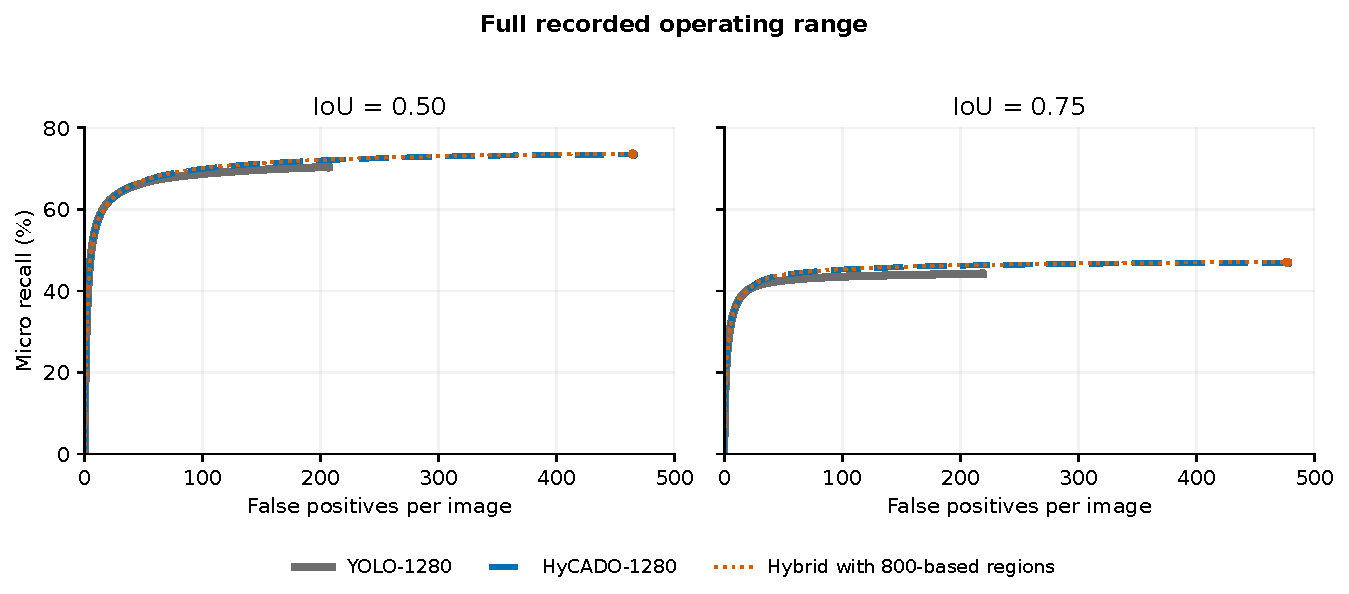
\includegraphics[width=\textwidth]{figures/recall_testdev_full.pdf}
\caption{Full recorded test-dev recall--FP range under toolkit-aligned max500 matching. Curves end at actual archived-score coverage, without extrapolation. The main article uses the same retained curve data on a common linear-near-zero/logarithmic-above-0.5 horizontal axis; the table resolves the prespecified low-FP budgets.}
\end{figure}
The largest whole pooled score prefix within each budget is selected separately per method and recomputed in each resample. FP counts can fall below a budget when the next tied group would exceed it. These are empirical operating points, not deployment thresholds. Crop scores cannot exceed 0.25 after scaling, while the measured low-FP cutoffs remain higher.

\section{Historical toolkit resolution results}
The following tables preserve the pre-COCO endpoint and must not be substituted for the COCO numbers. The 800-region variant uses original YOLO-800 crop selection and YOLO-1280 global predictions, with the same crop model and multiplier. Its separate proposal pass remains part of the complete configuration.
\begin{table}[h!]
\centering\footnotesize\setlength{\tabcolsep}{4pt}
\caption{Toolkit test-dev resolution extension. Macro AP is the equal-class toolkit diagnostic.}
\begin{tabular}{lrrrrr}
\toprule
Method & $\APlit$ & AP50 & AP75 & AR500 & Macro AP\\
\midrule
YOLO-1280 & 28.738 & 48.023 & 29.613 & 40.099 & 23.817\\
HyCADO-1280 (1280 regions + 1280 global) & 29.243 & 48.589 & 30.239 & 42.608 & 24.260\\
800 regions + 1280 global & 29.281 & 48.669 & 30.280 & 42.709 & 24.295\\
HyCADO-800 reference & 26.768 & 44.327 & 27.893 & 39.625 & 22.178\\
\bottomrule
\end{tabular}

\end{table}
\begin{table}[h!]
\centering\small
\caption{Toolkit AP contrasts for the resolution extension, with 1000 paired proxy-cluster draws.}
\begin{tabular}{lrr}
\toprule
Contrast & $\Delta$AP & 95\% interval\\
\midrule
1280 regions minus YOLO-1280 & +0.505 & [+0.129, +0.885]\\
800 regions minus YOLO-1280 & +0.544 & [+0.168, +0.924]\\
800 minus 1280 regions & +0.038 & [+0.004, +0.069]\\
\bottomrule
\end{tabular}

\end{table}
\clearpage
\begin{table}[h!]
\centering\small
\caption{Toolkit test-dev comparison including frozen SAHI-640. SAHI contrasts were bootstrapped only under the COCO definition.}
\begin{tabular}{lrrrr}
\toprule
Method & $\APlit$ & AP50 & AP75 & AR500\\
\midrule
YOLO-1280 & 28.738 & 48.023 & 29.613 & 40.099\\
HyCADO-1280 & 29.243 & 48.589 & 30.239 & 42.608\\
SAHI-640 + YOLO & 29.479 & 49.643 & 30.311 & 43.541\\
\bottomrule
\end{tabular}

\end{table}
\begin{table}[h!]
\centering\small\setlength{\tabcolsep}{5pt}
\caption{Class-wise toolkit AP for the resolution extension. Differences are relative to YOLO-1280.}
\begin{tabular}{lrrrrr}
\toprule
Class & YOLO-1280 & 1280 regions & 800 regions & $\Delta$1280 & $\Delta$800\\
\midrule
pedestrian & 19.221 & 19.532 & 19.592 & +0.311 & +0.371\\
people & 9.006 & 9.820 & 9.900 & +0.814 & +0.894\\
bicycle & 9.246 & 9.829 & 9.796 & +0.583 & +0.550\\
car & 53.089 & 53.761 & 53.754 & +0.672 & +0.664\\
van & 26.527 & 27.911 & 27.995 & +1.384 & +1.468\\
truck & 31.689 & 31.734 & 31.832 & +0.046 & +0.143\\
tricycle & 16.709 & 16.752 & 16.814 & +0.042 & +0.105\\
awning-tricycle & 9.807 & 10.448 & 10.442 & +0.641 & +0.635\\
bus & 42.872 & 42.477 & 42.466 & -0.395 & -0.406\\
motor & 20.007 & 20.333 & 20.355 & +0.326 & +0.348\\
\bottomrule
\end{tabular}

\end{table}
\section{Historical VAL operating-point diagnostics}
These tables compare HyCADO-800 (original v1) and YOLO-1280 on frozen predictions for 548 VAL images. They use class-aware full-image matching at each IoU, retaining at most 500 detections after ignore handling. Differences are HyCADO-800 minus YOLO-1280. Marginal 95\% percentile intervals use 2000 paired draws over 75 filename/hash proxy groups, without multiple-comparison correction.

The primary point is IoU 0.50 and at most two false positives per image on average, over all images and separately over the 99 images with 1--30 normal objects. The largest whole score prefix within the cap is selected independently per method and group, and recomputed in each draw. Equal scores remain tied.
\begin{table}[h!]
\centering\footnotesize\setlength{\tabcolsep}{4.5pt}
\caption{Historical VAL matched-budget recall. YOLO denotes YOLO-1280; HyCADO denotes HyCADO-800. FP/I is realized false positives per image and R is recall (\%).}
\begin{tabular}{lrrrrrrrr}
\toprule
Group & IoU & Cap & YOLO FP/I & HyCADO FP/I & YOLO R & HyCADO R & $\Delta$ & 95\% interval\\
\midrule
All VAL & 0.50 & 0.5 & 0.498 & 0.496 & 14.26 & 14.35 & $+0.08$ & $[-1.17, 1.30]$\\
 &  & 1 & 0.996 & 0.998 & 23.73 & 23.31 & $-0.42$ & $[-2.08, 1.24]$\\
 &  & 2 & 1.971 & 1.974 & 35.04 & 33.60 & $-1.44$ & $[-2.96, -0.15]$\\
 &  & 5 & 4.987 & 4.982 & 50.70 & 46.37 & $-4.33$ & $[-5.50, -3.05]$\\
 &  & 10 & 9.991 & 9.943 & 61.11 & 54.07 & $-7.04$ & $[-7.96, -5.75]$\\
 & 0.75 & 0.5 & 0.495 & 0.500 & 12.75 & 12.85 & $+0.10$ & $[-0.81, 0.72]$\\
 &  & 1 & 0.976 & 0.969 & 18.52 & 18.25 & $-0.27$ & $[-0.89, 0.50]$\\
 &  & 2 & 1.974 & 1.980 & 25.05 & 24.29 & $-0.76$ & $[-1.59, -0.06]$\\
 &  & 5 & 4.956 & 4.949 & 33.44 & 30.99 & $-2.45$ & $[-3.00, -1.68]$\\
 &  & 10 & 9.911 & 9.920 & 39.63 & 36.30 & $-3.34$ & $[-4.24, -2.49]$\\
1--30 GT objects & 0.50 & 0.5 & 0.495 & 0.495 & 40.54 & 34.86 & $-5.68$ & $[-13.00, 4.86]$\\
 &  & 1 & 0.990 & 1.000 & 50.10 & 51.19 & $+1.10$ & $[-3.44, 6.47]$\\
 &  & 2 & 1.980 & 2.000 & 59.72 & 62.30 & $+2.58$ & $[-2.34, 8.42]$\\
 &  & 5 & 5.000 & 5.000 & 68.62 & 69.66 & $+1.03$ & $[-3.99, 6.50]$\\
 &  & 10 & 10.000 & 10.000 & 73.47 & 75.15 & $+1.68$ & $[-2.66, 7.16]$\\
 & 0.75 & 0.5 & 0.475 & 0.485 & 29.70 & 28.28 & $-1.42$ & $[-4.28, 1.14]$\\
 &  & 1 & 1.000 & 1.000 & 38.02 & 37.06 & $-0.97$ & $[-3.65, 1.71]$\\
 &  & 2 & 2.000 & 1.939 & 43.12 & 43.83 & $+0.71$ & $[-2.44, 4.12]$\\
 &  & 5 & 4.990 & 4.990 & 50.36 & 52.23 & $+1.87$ & $[-2.35, 6.50]$\\
 &  & 10 & 10.000 & 10.000 & 53.71 & 57.20 & $+3.49$ & $[-0.50, 7.63]$\\
\bottomrule
\end{tabular}

\end{table}
\clearpage
\section{Historical VAL size and object-count diagnostics}
These tables use the original outputs up to global500, without matching false-positive rates. Normal targets are assigned to native-area bins after full-image matching. False positives have no GT area and are not assigned to these bins. These are stratified recall values, not area-specific AP. Object-count groups use the number of normal targets per image, not spatial density. Pooled precision is $\mathrm{TP}/(\mathrm{TP}+\mathrm{FP})$, excluding ignored detections. No evaluated image has zero normal targets and no retained normal target has nonpositive area.
\begin{table}[h!]
\centering\small\setlength{\tabcolsep}{6pt}
\caption{Historical VAL recall (R, \%) by native annotation area in pixels squared; GT is normal-target count. HyCADO is the 800 configuration.}
\begin{tabular}{llrrrrr}
\toprule
IoU & Area (px$^2$) & GT & YOLO R & HyCADO R & $\Delta$ & 95\% interval\\
\midrule
0.50 & $<256$ & 11844 & 66.08 & 63.42 & $-2.66$ & $[-5.29, 0.17]$\\
 & $[256,1024)$ & 14584 & 84.06 & 84.68 & $+0.62$ & $[-0.91, 2.12]$\\
 & $[1024,9216)$ & 11103 & 88.50 & 91.42 & $+2.92$ & $[2.31, 3.66]$\\
 & $\geq 9216$ & 1068 & 88.67 & 93.26 & $+4.59$ & $[1.89, 8.64]$\\
0.75 & $<256$ & 11844 & 25.54 & 25.44 & $-0.10$ & $[-1.37, 1.37]$\\
 & $[256,1024)$ & 14584 & 54.81 & 54.15 & $-0.66$ & $[-1.78, 0.68]$\\
 & $[1024,9216)$ & 11103 & 76.00 & 78.93 & $+2.94$ & $[2.09, 3.92]$\\
 & $\geq 9216$ & 1068 & 84.74 & 89.79 & $+5.06$ & $[2.25, 9.36]$\\
\bottomrule
\end{tabular}

\end{table}
\begin{table}[h!]
\centering\footnotesize\setlength{\tabcolsep}{4pt}
\caption{Historical VAL recall difference, pooled precision, and FP counts by object count. Differences are HyCADO-800 minus YOLO-1280.}
\begin{tabular}{llrrrrrrrr}
\toprule
IoU & GT/image & Images & GT & $\Delta$R & 95\% interval & YOLO P & HyCADO P & YOLO FP & HyCADO FP\\
\midrule
0.50 & 1--30 & 99 & 1549 & $+7.30$ & $[3.16, 11.97]$ & 13.43 & 2.76 & 7927 & 47286\\
 & 31--100 & 343 & 22316 & $+2.11$ & $[1.31, 3.02]$ & 16.24 & 10.85 & 93470 & 152730\\
 & 101 or more & 106 & 14734 & $-2.95$ & $[-4.44, -1.52]$ & 22.59 & 20.90 & 39448 & 41924\\
0.75 & 1--30 & 99 & 1549 & $+7.94$ & $[4.10, 12.20]$ & 9.63 & 2.07 & 8275 & 47624\\
 & 31--100 & 343 & 22316 & $+1.68$ & $[0.87, 2.53]$ & 10.90 & 7.32 & 99428 & 158782\\
 & 101 or more & 106 & 14734 & $-1.54$ & $[-2.31, -0.68]$ & 14.36 & 13.38 & 43641 & 45909\\
\bottomrule
\end{tabular}

\end{table}
\clearpage
\section{Two-resolution fusion and multiplier sensitivity}
The completed two-resolution control uses the frozen YOLO-800 and YOLO-1280 final outputs in native coordinates, unchanged scores, class-wise NMS at IoU 0.7, and a global cap of 1000. The primary recorded contrast is HyCADO-1280 minus fusion. Its paired draws reuse the exact 61 proxy groups, draw identities, and comparator values from the earlier analyses. The secondary contrasts are marginal and unadjusted. This control followed earlier test-dev results and does not establish an equal-compute ordering.
\begin{table}[h!]
\centering\small\setlength{\tabcolsep}{4pt}
\caption{Two-resolution YOLO fusion on all 1610 test-dev images, COCO-style point metrics.}
\begin{tabular}{rrrrrrrr}
\toprule
maxDets & AP & AP$_{50}$ & AP$_{75}$ & AP$_S$ & AP$_M$ & AP$_L$ & AR\\
\midrule
100 & 25.311 & 42.027 & 26.055 & 15.661 & 35.160 & 43.238 & 39.520\\
500 & 25.432 & 42.391 & 26.108 & 15.785 & 35.283 & 43.236 & 40.138\\
\bottomrule
\end{tabular}

\end{table}
\begin{table}[h!]
\centering\small\setlength{\tabcolsep}{4pt}
\caption{Paired differences for the completed fusion control, maxDets100. Intervals are 95\% percentile intervals conditional on the retained trained models.}
\begin{tabular}{llrr}
\toprule
Contrast & Metric & $\Delta$ & 95\% interval\\
\midrule
HyCADO-1280 $-$ fusion & AP & -0.876 & [-1.506, -0.152]\\
HyCADO-1280 $-$ fusion & AP50 & -1.223 & [-2.152, -0.116]\\
HyCADO-1280 $-$ fusion & AP75 & -1.115 & [-1.828, -0.261]\\
HyCADO-1280 $-$ fusion & AR100 & -0.392 & [-1.275, +0.954]\\
Fusion $-$ YOLO-1280 & AP & +1.315 & [+0.837, +1.919]\\
Fusion $-$ YOLO-1280 & AP50 & +1.797 & [+1.076, +2.605]\\
Fusion $-$ YOLO-1280 & AP75 & +1.631 & [+1.014, +2.404]\\
Fusion $-$ YOLO-1280 & AR100 & +3.353 & [+2.735, +4.262]\\
Fusion $-$ SAHI-640 & AP & +0.782 & [+0.195, +1.398]\\
Fusion $-$ SAHI-640 & AP50 & +0.404 & [-0.521, +1.509]\\
Fusion $-$ SAHI-640 & AP75 & +1.134 & [+0.435, +1.757]\\
Fusion $-$ SAHI-640 & AR100 & -0.297 & [-0.831, +0.173]\\
\bottomrule
\end{tabular}

\end{table}
\clearpage
The raw-query audit verifies all 1610 archive hashes and exactly reconstructs the original HyCADO-800, HyCADO-1280, and 800-region/1280-global outputs. The subsequent multiplier grid keeps the raw-score cutoff, coordinates, crop plans, global scores, sorting, NMS, and output cap fixed. Positive values rerank and fuse the full candidate lists; zero disables the crop branch and reuses the original global endpoint. No new confidence intervals are computed for this descriptive grid, and the original multiplier is retained.
\begin{table}[h!]
\centering\small\setlength{\tabcolsep}{4pt}
\caption{Complete multiplier sensitivity on test-dev. The original $\alpha=0.25$ reproduces the prior COCO result exactly. No optimal multiplier is selected from this previously examined split.}
\begin{tabular}{rrrrrrrrr}
\toprule
$\alpha$ & maxDets & AP & AP$_{50}$ & AP$_{75}$ & AP$_S$ & AP$_M$ & AP$_L$ & AR\\
\midrule
0 & 100 & 23.996 & 40.230 & 24.425 & 15.365 & 33.295 & 35.016 & 36.166\\
0 & 500 & 24.085 & 40.521 & 24.455 & 15.454 & 33.426 & 35.139 & 36.529\\
0.125 & 100 & 24.510 & 41.043 & 24.972 & 15.897 & 33.947 & 35.022 & 39.376\\
0.125 & 500 & 24.641 & 41.392 & 25.032 & 16.035 & 34.082 & 35.206 & 40.375\\
0.25 & 100 & 24.435 & 40.804 & 24.940 & 15.906 & 33.832 & 34.910 & 39.128\\
0.25 & 500 & 24.564 & 41.138 & 25.012 & 16.047 & 33.940 & 34.996 & 40.144\\
0.5 & 100 & 24.189 & 40.071 & 24.827 & 15.803 & 33.535 & 34.834 & 38.771\\
0.5 & 500 & 24.314 & 40.416 & 24.894 & 15.941 & 33.623 & 34.847 & 39.806\\
1 & 100 & 22.256 & 36.356 & 23.121 & 14.797 & 31.473 & 34.042 & 38.284\\
1 & 500 & 22.383 & 36.685 & 23.185 & 14.955 & 31.543 & 34.087 & 39.390\\
\bottomrule
\end{tabular}

\end{table}

\section{Matched crop-geometry diagnostics}
These counts describe the original HyCADO-1280 at $\alpha=0.25$. Source crop/query IDs are retained through exact NMS, ignore filtering, and COCO's own detection-ID matching. The population is the per-image, per-class top100 after the pinned ignore filter, with area set to all. The display subgroup additionally requires scaled score at least 0.05. Area ratio is decoded box area divided by originating crop area. The raw audit had no ignore filtering or COCO cap, so its 4676 crop-filling display boxes and the evaluated subset of 4534 have different populations. A COCO FP can be a duplicate or a class/localization error; these counts do not identify an AP contribution or a causal artefact effect.
\begin{table}[h!]
\centering\footnotesize\setlength{\tabcolsep}{4pt}
\caption{Crop-source detections by box/crop area ratio, class-aware COCO matches. Precision is $\mathrm{TP}/(\mathrm{TP}+\mathrm{FP})$ within each diagnostic subset; it is not AP. No box-removal counterfactual or uncertainty interval was computed.}
\begin{tabular}{llrrrr}
\toprule
IoU & Crop subset & TP & FP & Ignored & Precision (\%)\\
\midrule
0.5 & All crop & 4274 & 542731 & 0 & 0.781\\
0.5 & Area ratio $\geq0.95$ & 2 & 8498 & 0 & 0.024\\
0.5 & Area ratio $<0.95$ & 4272 & 534233 & 0 & 0.793\\
0.5 & Display-score crop & 2802 & 46676 & 0 & 5.663\\
0.5 & Display, ratio $\geq0.95$ & 0 & 4534 & 0 & 0.000\\
0.5 & Display, ratio $<0.95$ & 2802 & 42142 & 0 & 6.234\\
0.75 & All crop & 2536 & 544469 & 0 & 0.464\\
0.75 & Area ratio $\geq0.95$ & 1 & 8499 & 0 & 0.012\\
0.75 & Area ratio $<0.95$ & 2535 & 535970 & 0 & 0.471\\
0.75 & Display-score crop & 1839 & 47639 & 0 & 3.717\\
0.75 & Display, ratio $\geq0.95$ & 0 & 4534 & 0 & 0.000\\
0.75 & Display, ratio $<0.95$ & 1839 & 43105 & 0 & 4.092\\
\bottomrule
\end{tabular}

\end{table}
\clearpage
\section{Geometric properties of the fixed merge}
Let $\mathcal R_0=(r_i^{(0)})_{i=0}^{n-1}$ be the initial distinct expanded rectangles. Each active cluster stores member indices and its hull. Singleton initialization partitions the indices. Replacing two clusters by their hull, and coalescing identical hulls, preserves that partition and contains every initial member. Each operation reduces active count, so at most $\max(n-1,0)$ merges occur. For final crops $r_1,\ldots,r_{m(I)}$,
\[
0\leq m(I)\leq n\leq60,\qquad
\bigcup_{i=0}^{n-1}r_i^{(0)}\subseteq\bigcup_{j=1}^{m(I)}r_j.
\]
Hulls may add background; the soft target of ten does not force merging after all eligible pairs are exhausted. The growth test compares hull dimensions with minimum width and height of \emph{initial} members. If initial rectangle $i$, with dimensions $w_i,h_i$, belongs to final crop $j$, with dimensions $w_j,h_j$, crop side $L=960$ and tolerance $\varepsilon=10^{-12}$ give
\[
\frac{L/w_j}{L/w_i}=\frac{w_i}{w_j}\geq\frac1{3+\varepsilon},\qquad
\frac{L/h_j}{L/h_i}=\frac{h_i}{h_j}\geq\frac1{3+\varepsilon}.
\]
Carrying initial-member minima forward controls enlargement accumulated across merges. The bound concerns geometric resize scale, not recognition accuracy. Each crop adds at most 300 candidates, giving at most $1000+300m(I)\leq19000$ before fusion. Final NMS and truncation can remove candidates, so containment does not guarantee preservation of YOLO recall.

\section{Qualitative sampling and display protocol}
The twelve-image test-dev sample uses seed 20261112. For each image the SHA256 digest is calculated from the UTF-8 string
\begin{center}\texttt{20261112|group\_label|image\_path}\end{center} Images are ranked by increasing digest, retaining the first occurrence of each distinct filename proxy group until twelve groups are represented. The first three form the main figure. This rule does not yield equal group-selection probabilities or verified independent scenes. Image selection was fixed before these qualitative outputs were viewed; the underlying split had been examined numerically.

After the pinned ignore filter, candidate centers use up to 100 evenly spaced annotation-order indices of normal GT. Each $640\times420$ window is translated to fit the image. The window with the most normal-GT centers is retained, with ties favoring smaller $x$, then smaller $y$. GT affects only the display window. Archived scores and coordinates are preserved, with display score $\geq0.05$, no added NMS, and no candidate cap. Colors identify classes, not matching status. Crossing boxes are clipped only for rendering. The common threshold does not calibrate scores or equalize FP rates.

The following twelve-page atlas retains all selected examples, including the three main rows. Original image context, window, and detector outputs appear together. Image, annotation, and selected prediction-payload hashes were verified against retained sources. No source databases were changed.
\clearpage
\includepdf[pages=-,pagecommand={\thispagestyle{empty}},fitpaper=false]{qualitative1280_supplementary.pdf}
\end{document}
